	
\documentclass[letterpaper, 11pt]{extarticle}
% \usepackage{fontspec}

% ==================================================

% document parameters
% \usepackage[spanish, mexico, es-lcroman]{babel}
\usepackage[english]{babel}
\usepackage[margin = 1in]{geometry}

% ==================================================

% Packages for math
\usepackage{mathrsfs}
\usepackage{amsfonts}
\usepackage{amsmath}
\usepackage{amsthm}
\usepackage{amssymb}
\usepackage{physics}
\usepackage{dsfont}
\usepackage{esint}

% ==================================================

% Packages for writing
\usepackage{enumerate}
\usepackage[shortlabels]{enumitem}
\usepackage{framed}
\usepackage{csquotes}

% ==================================================

% Miscellaneous packages
\usepackage{float}
\usepackage{tabularx}
\usepackage{xcolor}
\usepackage{multicol}
\usepackage{subcaption}
\usepackage{caption}
\captionsetup{format = hang, margin = 10pt, font = small, labelfont = bf}

% Citation
\usepackage[round, authoryear]{natbib}

% Hyperlinks setup
\usepackage{hyperref}
\definecolor{links}{rgb}{0.36,0.54,0.66}
\hypersetup{
   colorlinks = true,
    linkcolor = black,
     urlcolor = blue,
    citecolor = blue,
    filecolor = blue,
    pdfauthor = {Author},
     pdftitle = {Title},
   pdfsubject = {subject},
  pdfkeywords = {one, two},
  pdfproducer = {LaTeX},
   pdfcreator = {pdfLaTeX},
   }
\usepackage{titlesec}
\usepackage[many]{tcolorbox}

% Adjust spacing after the chapter title
% \titlespacing*{<command>}{<left>}{<before-sep>}{<after-sep>}
\titlespacing*{\chapter}{0cm}{-2.0cm}{0.50cm}
\titlespacing*{\section}{0cm}{0.50cm}{0.25cm}

% Indent 
\setlength{\parindent}{0pt}
\setlength{\parskip}{1ex}

% --- Theorems, lemma, corollary, postulate, definition ---
% \numberwithin{equation}{section}


\newtcbtheorem[]{problem}{Problem}%
    {enhanced,
    colback = black!5, %white,
    colbacktitle = black!5,
    coltitle = black,
    boxrule = 0pt,
    frame hidden,
    borderline west = {0.5mm}{0.0mm}{black},
    fonttitle = \bfseries\sffamily,
    breakable,
    before skip = 3ex,
    after skip = 3ex
}{problem}

\tcbuselibrary{skins, breakable}
%%% Commands defined by me
%   Euler constant
\newcommand{\eu}{\mathrm{e}}

%   Imaginary unit
\newcommand{\im}{\mathrm{i}}

%   Degrees
\newcommand{\grado}{\,^{\circ}}

%%% Linear Algebra

% Transpose
\newcommand{\transpose}[1]{{#1}^{\mathsf{T}}}

%%% Calculus
%   Integral from - infinity to infinity 
\newcommand{\Int}{\int\limits_{-\infty}^{\infty}}

%   Indefinite integral
\newcommand{\rint}[2]{\int{#1}\dd{#2}}

%   Definite integral
\newcommand{\Rint}[4]{\int\limits_{#1}^{#2}{#3}\dd{#4}}


% Serif bold text
\newcommand{\tsb}[1]{\textsf{\textbf{#1}}}

% Separation line
\newcommand{\linea}{\textcolor{gray!60}{\rule{\linewidth}{0.2pt}}}

% Bigger version of a \cdot to denote dot product
\makeatletter
\newcommand*\bigcdot{\mathpalette\bigcdot@{.5}}
\newcommand*\bigcdot@[2]{\mathbin{\vcenter{\hbox{\scalebox{#2}{$\m@th#1\bullet$}}}}}
\makeatother

% My Hamiltonian prefered notation
\newcommand{\Ham}{\hat{\mathcal{H}}}

%% Pre-existing commands redefined by me
% Trace of a matrix 
\renewcommand{\Tr}{\mathrm{Tr}}



\begin{document}
		\begin{Large}
		\textsf{\textbf{Characterisation of domain of attraction}}\\
		Section 10 - Home Work 2
	\end{Large}
	
	\vspace{1ex}
	
	\textsf{\textbf{Student:}} \text{Mehrab Atighi}, \href{mailto:mehrab.atighi@gmail.com}{\texttt{mehrab.atighi@gmail.com}}\\
	\textsf{\textbf{Lecturer:}} \text{Mohammad Zokaei}, \href{mailto:Zokaei@sbu.ac.ir}{\texttt{Zokaei@sbu.ac.ir}}
	
	
	\vspace{2ex}
	
	\begin{problem}{}{problem-label}
			\textbf{Theorem 2.2.8 (Characterisation of domain of attraction)}
		
		\begin{itemize}
			\item[(b)] The df \( F \) belongs to the domain of attraction of an \(\alpha\)-stable law for some \(\alpha < 2\) if and only if
			
			
			\[
			F(-x) = \frac{c_1 + o(1)}{x^\alpha} L(x), \quad 1 - F(x) = \frac{c_2 + o(1)}{x^\alpha} L(x), \quad x \to \infty,
			\]
			
			
			where \( L \) is slowly varying and \( c_1, c_2 \) are non-negative constants such that \( c_1 + c_2 > 0 \).
		\end{itemize}
		\cite{Embrechts.etal1997}:
	\end{problem}
	
	\begin{solve}{}{solve-label}
\textbf{Proof:}

Consider a sequence of i.i.d. random variables \( X_1, X_2, \ldots, X_n \) with distribution function \( F \). We want to show that \( F \) belongs to the domain of attraction of an \(\alpha\)-stable law with \( \alpha < 2 \) if and only if the tails of \( F \) satisfy: \[ F(-x) = \frac{c_1 + o(1)}{x^\alpha} L(x) \quad \text{and} \quad 1 - F(x) = \frac{c_2 + o(1)}{x^\alpha} L(x), \quad x \to \infty, \] where \( L(x) \) is slowly varying and \( c_1, c_2 \geq 0 \) with \( c_1 + c_2 > 0 \). \\
\subsection*{Step 1: Tail Behavior and Characterization} For \( F \) to be in the domain of attraction of an \(\alpha\)-stable law, the tails of the distribution function \( F \) must have the form: \[ F(-x) \sim \frac{c_1}{x^\alpha} L(x) \quad \text{and} \quad 1 - F(x) \sim \frac{c_2}{x^\alpha} L(x), \quad \text{as } x \to \infty, \] where \( L(x) \) is a slowly varying function. This condition ensures that the distribution \( F \) has heavy tails, which is a characteristic of \(\alpha\)-stable distributions. \\
\subsection*{Step 2: Normalizing Constants} For a random variable \( X \) with distribution function \( F \), we need to show that for large \( n \), \[ \frac{S_n - a_n}{b_n} \xrightarrow{d} X, \] where \( S_n = X_1 + X_2 + \cdots + X_n \), and \( a_n \) is centering constant and \( b_n \) is normalizing constants. Using properties of \(\alpha\)-stable laws, we can choose \( b_n = n^{1/\alpha} \) and \( a_n = 0 \). \\
\subsection*{Step 3: Slowly Varying Function \( L(x) \)} A function \( L(x) \) is slowly varying at infinity if for any \( t > 0 \), \[ \lim_{x \to \infty} \frac{L(tx)}{L(x)} = 1. \] This definition implies that \( L(x) \) grows very slowly compared to any polynomial function. In our context, \( L(x) \) modulates the tail behavior of the distribution \( F \). \\
\subsection*{Step 4: Convergence of Normalized Sums} To conclude, if \( F \) has the specified tail behavior, then the normalized sum \( \frac{S_n}{n^{1/\alpha}} \) converges in distribution to an \(\alpha\)-stable law. This implies that \( F \) is in the domain of attraction of the \(\alpha\)-stable law. For large \( n \), consider: \[ P\left( \frac{S_n}{n^{1/\alpha}} \leq x \right) \approx F\left( x n^{1/\alpha} \right). \] Using the tail behavior of \( F \): \[ F\left( x n^{1/\alpha} \right) \sim \frac{c_1}{(x n^{1/\alpha})^\alpha} L(x n^{1/\alpha}) + \frac{c_2}{(x n^{1/\alpha})^\alpha} L(x n^{1/\alpha}). \] Since \( L(x) \) is slowly varying, \[ \frac{L(x n^{1/\alpha})}{L(n^{1/\alpha})} \to 1 \quad \text{as} \quad n \to \infty. \] Thus, \[ F\left( x n^{1/\alpha} \right) \sim \frac{c_1 + c_2}{x^\alpha} L(n^{1/\alpha}), \] which implies that \[ P\left( \frac{S_n}{n^{1/\alpha}} \leq x \right) \to G(x), \] where \( G(x) \) is the distribution function of an \(\alpha\)-stable law. Therefore, \( F \) is in the domain of attraction of an \(\alpha\)-stable law if the tails of \( F \) have the specified form with a slowly varying function \( L(x) \). Thus, we have shown that the second moment being slowly varying is a necessary condition for a distribution to be in the domain of attraction of the normal law.\\
i try to use \cite{r8}  for this proof. In the following you can see two page of this book.

\includegraphics[width = \textwidth]{pic1.png}
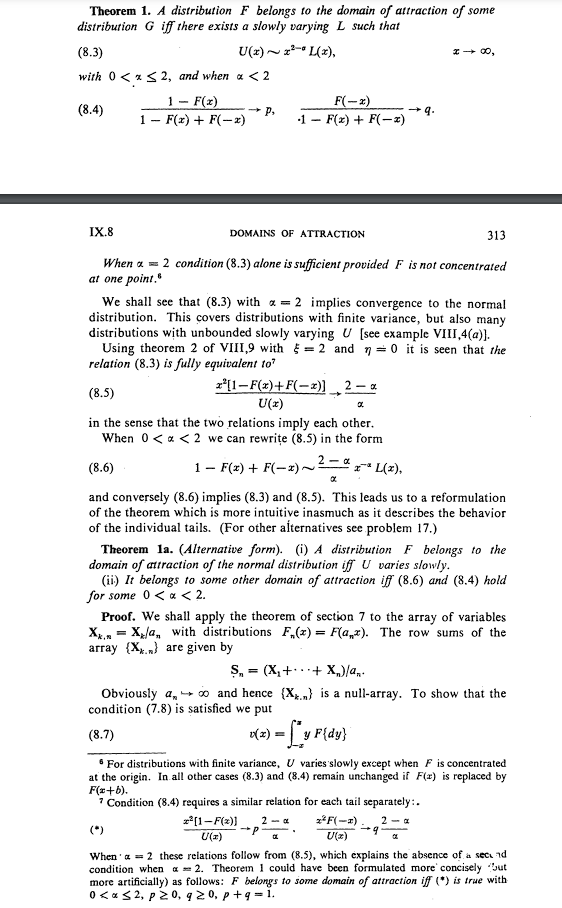
\includegraphics[width = \textwidth]{pic2.png}
 \cite{r1,r2,r3,r4,r5,r6,r7}
	\end{solve}
	% =================================================
	
	% \newpage
	
	% \vfill
	
	\bibliographystyle{apalike}
	\bibliography{references}
\end{document}